\chapter{Deep Learning in Digital Histopathology}

In this chapter, we begin by introducing the field of histopathology and its concerns, alongside with tools and methods used in contemporary clinical practice. We show how digitization helped to reduce the temporal and spatial complexity of everyday tasks, and how decision support systems can further reduce the human labor. We introduce artificial neural networks, with focus on convolutional networks, which are exceptional at tackling various computer vision problems.

\section{Histopathology}

Histopathology is a discipline concerned with study of diseases of tissue. This involves, but is not limited to cancer detection and prediction [], infectious or inflammatory disease diagnostics [] and study of brain-degenerative diseases such as Parkinson's or Alzheimer's [].

Histopathologists are medically qualified physicians, who inspect tissue extracted from patients. They are responsible for interpreting cellular abnormalities and tissue anomalies, that may signify various medical conditions. Histopathologists often cooperate with other doctors, to help set the direction of patients care [].

\section{Temporal and spatial limitations of traditional approach}

Traditionally, to get tissue from patient to histopathologist, tedious process involving several people is necessary. Tissue needs to be extracted from patient. Then it needs to be sent to specialized laboratory for further processing. In lab, tissue samples are infused with mix of chemicals and then infiltrated with paraffin wax, afterwards rest overnight. The next day, tissue is embedded into paraffin wax block and thinly sliced. Sliced sections of approx. $3$ microns are then put into a water bath to straighten, after which they are laminated into a glass slide. Glass slides are further stained with hematoxilin/eosin (or other compound) [] to enhance contrast between different cellular structures. Slides are then delivered to histopathologist for a review.

While we currently cannot replace ... performing the biopsy of lab worker staining and embedding the tissue, we can address logistic challenges of having a glass slides. Having a physical slide suffers from several inefficiencies. A slide can be studied only by one histopathologist at a time and if a second opinion from a different histopathologist is required, the glass slide must be conveyed to the respective clinic. This throttles the diagnosis process and leads to longer waiting times for a patient.

\section{Digital histopathology}

Digital histopathology aims to reduce the logistic overhead introduced by physical copies of glass slides. After the tissue is extracted and prepared, it is scanned using specialized lenses resulting in a high-resolution digital image, called \emph{Whole Slide Image} (WSI) [].

This image is then uploaded to an aggregator server, which enable real-time sharing of slides and parallel cooperation of multiple clinicians. Histopathologists then inspect WSI in a dedicated browsers on their computer monitors.

\todo{xopat screenshot}

Recently, researches and various companies made attempts to employ machine learning systems to further aid pathologist during the diagnosis process. 

\subsection*{Decision Support System}

A computer system, which aids human to make a decision while performing a particular task is referred to as decision support system []. These systems are utilized across a wide array of applications, including high-stake environments such as investment banking [], autonomous driving [] or military and defense []. In digital histopathology, such systems are usually utilized to help with operational processes []. With deep learning in the spotlight of today's research, new possibilities emerge.

New systems could be utilized to enhance tissue diagnostic process by assisted diagnosis, or used to discover previously unrecognized features in large sets of data, incomprehensible by a single expert [].

%% https://pathsocjournals.onlinelibrary.wiley.com/doi/10.1002/path.5388

Random forests [], support vector machines [] and various neural network architectures [] are all attempts of such utilization. Those systems often provide real-time results and human-like performance, demonstrating that further research in this area can bring significant improvement to the contemporary processes [].

%% decision trees - https://www.researchgate.net/publication/363350224_Random_forest_modelling_demonstrates_microglial_and_protein_misfolding_features_to_be_key_phenotypic_markers_in_C9orf72-ALS
%% svm - https://www.ncbi.nlm.nih.gov/pmc/articles/PMC1924513/pdf/1471-2121-8-S1-S8.pdf
%% neural networks - https://arxiv.org/pdf/2312.02225.pdf
%%                 - https://www.sciencedirect.com/science/article/pii/S2666827021000992

\section{Deep Learning}
%% Brief intro to what is deep learning, methods and techniques? Common use cases of deep learning in digital histopathology.

Area of machine learning encapsulating neural networks is referred to as deep learning (DL). Methods and algorithms employed by deep learning achieve remarkable results across various domains, including computer vision [imagenet?], games [alphago], weather forecast [] or natural language processing [gpt].

Introduced in 1943 by McCulloch and Pitts [] with goal of creating a computational unit resembling a neuron in human brain, neural networks have come a long way to the prominent place they occupy today.

%% forecast - https://www.nature.com/articles/s41586-023-06185-3

\subsection*{Neural Network}

A multi-layer perceptron is a simple feed-forward neural network. It can be seen as a function $f$ that maps real-valued input vector \textbf{x} to a single value $\hat{y}$. As the name suggest, a multi-layer perceptron is organized into layers and each layer consists of its trainable weights and biases, commonly in form of a real-valued matrices. Additionally, each layer has its activation function\footnote{Heaviside step function was the first activation function to be used. This led to a number of problems [] and because of their importance, activation functions are vital part of research interest up to this day [].}, usually denoted as $\Theta$. Formula for a function $f_l$ computed by a layer $l$ with weights $w_l$, biases $b_l$ and activation function $\Theta_l$ is denoted as:

\begin{equation}
\hat{y_l} = \Theta_l(w_l \cdot x + b_l)
\end{equation}
where $\hat{y_l}$ is output of the layer $l$, or simply $f_l(x)$.



Even though ... shows that one hidden layer is all you need to essentially approximate arbitrary function, artificial neural networks often consists of multiple layers. The motivation is that each layer can be seen as if it captures certain abstractions or patterns from its input. Deeper layers can build more complicated patterns utilizing abstractions captured by previous layers. Figure \ref{fig:simple-mlp} depicts a simple multi-layered perceptron (MLP) with one hidden layer.

Deep learning aims to make networks weights and biases useful. Since a network computes a function $f$, with specific training, we can make network learn to approximate any desited function $f*$ within a certain tolerance.

To achieve this, training leverages large amount of data to adjust networks parametes to minimize difference between its and desired outputs. This process is typically performed iteratively using loss function, backpropagation, and traning algorithm such as stochastic gradient descent. More on neural networks training can be found in [].

%% goodfellow kniha

\begin{figure}[!h]
    \begin{center}
    \begin{minipage}{.75\textwidth}
      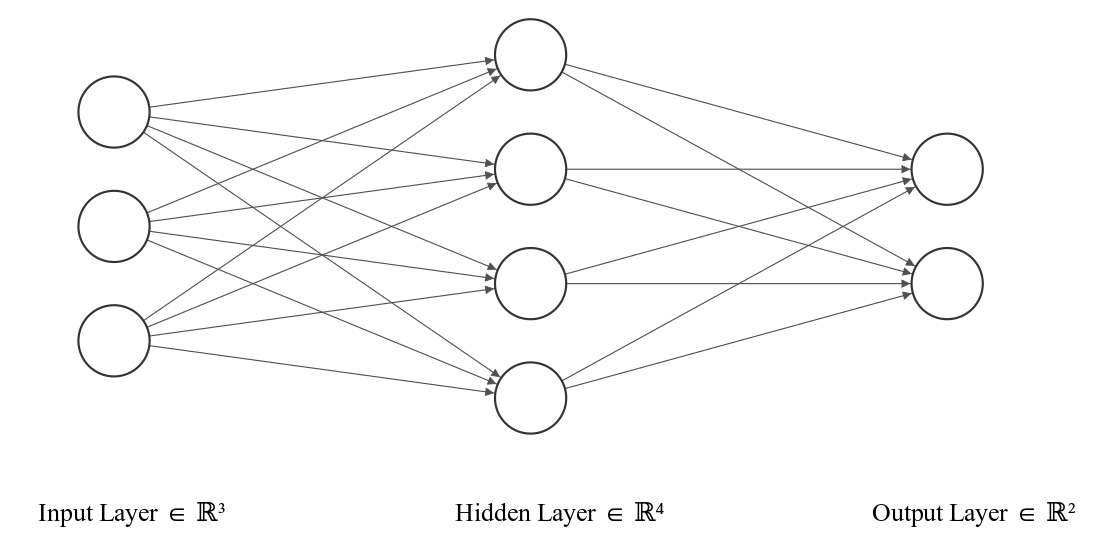
\includegraphics[width=\textwidth]{img/nn.png}
    \end{minipage}
    \caption{Architecture of a multi-layer perceptron with one hidden layer. Circles represent layer inputs. Edges represent layer weights. Biases are omitted for simplicity. Given a non-input layer L, if every unit has an incoming edge from all units in previous layer, we consider the perceptron to be fully-connected.}
    \label{fig:simple-mlp}
    \end{center}
\end{figure}

Despite MLP's demonstrating impressive results on tasks previously considered as impossible for computers, they come with some setbacks. Given they are fully connected, even small contemporary architectures such as ImageNET with multiple layers would have unimaginable number of trainable parameters. This led to development of new architectures, tailored to specific domain needs. Despite shift from using fully-connected layers only, MLP stood its ground and to this day, it is essential part of various state of the art neural network models [gpt, alexnet].

\subsection*{Convolutional Neural Network}
%% Architecture
Architecture introduced specifically to solve various computer vision problems adds two additional layer types --- convolutional and pooling. These layers help to capture features from input image, as well as reduce size of the network []. 
%% - https://arxiv.org/pdf/1511.08458.pdf

%% TODO: Why it suits them for image processing

\subsubsection{Convolutional Layer}

Convolutional layer works similar as to layers in a MLP. It utilizes learnable filters (alternatively called kernels) to search for patterns in its input.

Typically, a filter has significantly smaller dimensions compared to the input. Instead of interacting with whole input at once, as it is case for fully-connected layers, the filter is systematically slid across the input. Weights of a filter are convolved with the corresponding input data segments. This yields an activation map, which can be seen as a evidence for presence of a shape, detected by the filter in the input data.

When defining a convolutional layer, aside from filter shape, we need to supply two additional parameters, usually called \emph{padding} and \emph{stride}. Padding is used at the borders of the input feature map, to help prevent loss of information, where the filter could not be otherwise applied. Stride controls how much we shift the filter upon calculating one convolution. See Figure \ref{fig:cnn-convolution} for visualization.

\begin{figure}[!h]
    \begin{center}
    \begin{minipage}{0.75\textwidth}
      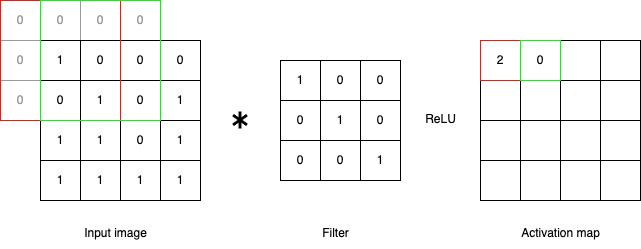
\includegraphics[width=\textwidth]{img/cnn-conv.png}
    \end{minipage}
    \caption{Example of simple calculation within convolution layer. Filter detects diagonal edge of lenght 3 pixels. Stride and padding are both set to 1 pixel and zero is used as the padded value. The result is passed through ReLU activation function.}
    \label{fig:cnn-convolution}
    \end{center}
\end{figure}

It is important to note, that a filter shares its weights with every input segment it attributes to. This gives us spatial in-variance -- meaning the filter is able to detect learned pattern at any position in the input features. Moreover, it drastically reduces the number of weights. Given $512$ input and output features, fully connected layers would need $262144$ weights. Simple $3x3$ filter needs $9$.

Traditionally, a convolutional layer consists of multiple filters. The idea is, that each filter is trained to activate upon seeing a different pattern. Given a one layer can detect multiple shapes, as outlined in section ..., it allows the deeper layers of network to combine simple patterns into more complex ones.

\subsubsection{Pooling Layer}

To prevent overfitting, pooling layers are employed to further distill patterns captured by a CNN. They progressively reduce size of the features, leading to reduced number of model parameters and computational complexity [].

A pooling layer is commonly placed after a convolutional one, iterating over its activation maps. It has its own filters and strides, however, the parameters are chosen more conservatively. Most of the time, filter is of size $2x2$ and stride is set to $2$, such that the pooled sectors do not overlap. It is reported that having a filter of size greater than 3 will most likely lead to loss of model's performance, since such granularity would hide more of the detected features [].

\begin{figure}[!h]
    \begin{center}
    \begin{minipage}{0.5\textwidth}
      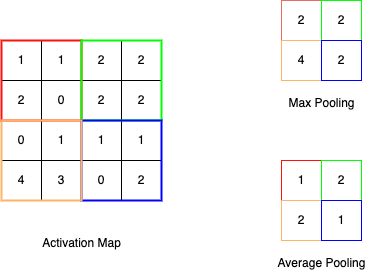
\includegraphics[width=\textwidth]{img/cnn-pool.png}
    \end{minipage}
    \caption{Example of both max and average pooling layers. Both have filters of size $2x2$ and stride set to $2$, resulting in no overlap during computation. Notice, that since each $2x2$ region is mapped to a single value, the new activation mask has quarter the features of the original.}
    \label{fig:cnn-pooling}
    \end{center}
\end{figure}
%%
